% Báo cáo bài tập nhóm – Các hệ thống phân tán – Nhóm 8
% Biên dịch: xelatex main.tex (chạy 2 lần) hoặc: latexmk -xelatex main.tex
\documentclass[12pt,a4paper,oneside]{report}

% ---------------------------------------------------------------- gói
\usepackage{fontspec}
\setmainfont{Times New Roman}
\setmonofont{Consolas}[Scale=0.88]
\usepackage[vietnamese]{babel}
\usepackage[left=3cm,right=2cm,top=2.5cm,bottom=2.5cm]{geometry}
\usepackage{graphicx}
\usepackage{xcolor}
\usepackage{tikz}
\usetikzlibrary{positioning,arrows.meta,shapes.geometric,calc,fit,backgrounds}
\usepackage{pgfornament}
\usepackage{eso-pic}
\usepackage{setspace}
\usepackage{titlesec}
\usepackage{fancyhdr}
\usepackage{booktabs}
\usepackage{tabularx}
\usepackage{longtable}
\usepackage{array}
\usepackage{multirow}
\usepackage{enumitem}
\usepackage{caption}
\usepackage{float}
\usepackage{listings}
\usepackage{fancyvrb}
\fvset{frame=single,framerule=0.4pt,rulecolor=\color{black!25},fontsize=\small,xleftmargin=4pt,xrightmargin=4pt,framesep=6pt}
\usepackage{amsmath}
\usepackage[hidelinks]{hyperref}

\definecolor{ptitred}{RGB}{204,31,36}
\definecolor{ptitdark}{RGB}{120,10,15}
\definecolor{codebg}{RGB}{246,246,246}
\definecolor{codegray}{RGB}{110,110,110}
\definecolor{codeblue}{RGB}{20,70,160}
\definecolor{codegreen}{RGB}{30,120,50}

\setstretch{1.3}
\setlength{\parskip}{4pt}
\setlength{\parindent}{1cm}
\setlist{itemsep=2pt,topsep=4pt}

% Tên thành viên – sửa ở đây nếu phân vai khác
\newcommand{\memberA}{Lương Sơn Tùng}
\newcommand{\memberAid}{B23DCVT448}
\newcommand{\memberB}{Ngô Minh Tùng}
\newcommand{\memberBid}{B23DCDT279}
\newcommand{\memberC}{Tạ Quang Vinh}
\newcommand{\memberCid}{B23DCDT289}

% ---------------------------------------------------------------- tiêu đề chương
\titleformat{\chapter}[display]
  {\centering\bfseries\color{ptitdark}}
  {\Large CHƯƠNG \thechapter}
  {6pt}
  {\LARGE\MakeUppercase}
\titlespacing*{\chapter}{0pt}{-10pt}{24pt}
\titleformat{\section}{\large\bfseries}{\thesection}{0.6em}{}
\titleformat{\subsection}{\normalsize\bfseries}{\thesubsection}{0.6em}{}
\titleformat{\subsubsection}{\normalsize\bfseries\itshape}{\thesubsubsection}{0.6em}{}

\captionsetup{font=small,labelfont=bf}
\addto\captionsvietnamese{%
  \renewcommand{\contentsname}{MỤC LỤC}%
  \renewcommand{\listfigurename}{DANH MỤC HÌNH VẼ}%
  \renewcommand{\listtablename}{DANH MỤC BẢNG BIỂU}%
  \renewcommand{\bibname}{TÀI LIỆU THAM KHẢO}%
  \renewcommand{\figurename}{Hình}%
  \renewcommand{\tablename}{Bảng}%
  \renewcommand{\chaptername}{Chương}%
}

\pagestyle{fancy}
\fancyhf{}
\fancyhead[L]{\small\itshape Các hệ thống phân tán -- Nhóm 8}
\fancyhead[R]{\small\itshape DS02 -- Hệ thống chia sẻ file P2P kiểu BitTorrent}
\fancyfoot[C]{\thepage}
\renewcommand{\headrulewidth}{0.4pt}
\fancypagestyle{plain}{\fancyhf{}\fancyfoot[C]{\thepage}\renewcommand{\headrulewidth}{0pt}}

\lstset{
  basicstyle=\ttfamily\small,
  backgroundcolor=\color{codebg},
  frame=single, rulecolor=\color{black!20},
  breaklines=true, columns=fullflexible, keepspaces=true,
  showstringspaces=false, tabsize=4,
  xleftmargin=4pt, xrightmargin=4pt, aboveskip=8pt, belowskip=8pt,
  commentstyle=\color{codegreen}\itshape,
  keywordstyle=\color{codeblue}\bfseries,
  stringstyle=\color{ptitred},
  extendedchars=true, inputencoding=utf8,
}
\lstdefinelanguage{yaml}{keywords={true,false},sensitive=false,comment=[l]{\#},morestring=[b]"}
\lstdefinelanguage{json}{morestring=[b]",literate={:}{{\textcolor{codegray}{:}}}1}

\newcolumntype{L}{>{\raggedright\arraybackslash}X}

% ================================================================= tài liệu
\begin{document}

% ----------------------------------------------------------------- BÌA
\begin{titlepage}
\thispagestyle{empty}
\AddToShipoutPictureFG*{%
  \begin{tikzpicture}[remember picture,overlay]
    % khung đôi: viền ngoài tô kín (even-odd) để 4 cạnh dày đúng bằng nhau
    \fill[black,even odd rule]
      ($(current page.north west)+(2.2cm,-1.7cm)$) rectangle ($(current page.south east)+(-1.5cm,1.7cm)$)
      ($(current page.north west)+(2.3cm,-1.8cm)$) rectangle ($(current page.south east)+(-1.6cm,1.8cm)$);
    \draw[line width=0.7pt,color=black]
      ($(current page.north west)+(2.45cm,-1.95cm)$) rectangle ($(current page.south east)+(-1.75cm,1.95cm)$);
  \end{tikzpicture}}
\begin{center}
  \vspace*{0.4cm}
  {\large\bfseries HỌC VIỆN CÔNG NGHỆ BƯU CHÍNH VIỄN THÔNG}\\[2pt]
  {\large\bfseries KHOA CÔNG NGHỆ THÔNG TIN 1}\\[2pt]
  \rule{4.5cm}{0.6pt}\\[1.0cm]

  
\includegraphics[width=3.6cm]{images/logo-ptit.png}\\[1.3cm]

  {\Large\bfseries BÁO CÁO BÀI TẬP NHÓM}\\[6pt]
  {\large\bfseries MÔN: CÁC HỆ THỐNG PHÂN TÁN}\\[0.9cm]

  {\color{ptitdark}\LARGE\bfseries ĐỀ TÀI DS02}\\[6pt]
  {\color{ptitdark}\Large\bfseries XÂY DỰNG HỆ THỐNG CHIA SẺ FILE NGANG HÀNG}\\[2pt]
  {\color{ptitdark}\Large\bfseries MÔ PHỎNG GIAO THỨC BITTORRENT}\\[1.4cm]

  \begin{tabular}{@{}l@{\hspace{1.2em}}l@{}}
    \textbf{Giảng viên hướng dẫn:} & \textbf{Kim Ngọc Bách}\\[6pt]
    \textbf{Nhóm thực hiện:} & \textbf{Nhóm 8}\\[4pt]
    & Tạ Quang Vinh \hfill B23DCDT289\\
    & Ngô Minh Tùng \hfill B23DCDT279\\
    & Lương Sơn Tùng \hspace{2.2em}\hfill B23DCVT448\\
  \end{tabular}

  \vfill
  {\large\bfseries Hà Nội -- 2026}
  \vspace*{0.6cm}
\end{center}
\end{titlepage}

% ----------------------------------------------------------------- PHẦN ĐẦU
\pagenumbering{roman}
\setcounter{page}{2}

\chapter*{LỜI NÓI ĐẦU}
\addcontentsline{toc}{chapter}{Lời nói đầu}

Trong môn Các hệ thống phân tán, nhóm em được giao đề tài DS02: xây dựng một hệ thống chia sẻ file ngang hàng (P2P) theo kiểu BitTorrent. Đây là đề tài khá ``đúng chất'' phân tán: không có một máy chủ nào giữ toàn bộ dữ liệu, mỗi máy vừa là người tải vừa là người phục vụ, các máy có thể vào ra hoặc sập bất cứ lúc nào, và hệ thống vẫn phải đảm bảo file tải về đúng từng byte.

Nhóm chọn Python để cài đặt vì viết nhanh, dễ đọc và có sẵn thư viện cho socket, HTTP và đa luồng. Ngoài phần lõi (tracker và peer), nhóm còn làm thêm bộ mô phỏng để bật hàng chục tiến trình peer, gây churn (peer vào/ra/sập), làm sập tracker, rồi đo đạc và vẽ biểu đồ. Nhờ vậy nhóm không chỉ ``chạy được'' mà còn đánh giá được hệ thống trong nhiều tình huống khác nhau.

Báo cáo gồm 6 chương: giới thiệu đề tài, cơ sở lý thuyết, thiết kế hệ thống, cài đặt từng module, kiểm thử và thực nghiệm, cuối cùng là kết luận. Do thời gian và kiến thức còn hạn chế nên báo cáo khó tránh khỏi thiếu sót, nhóm em rất mong nhận được góp ý của thầy để hoàn thiện hơn.

Nhóm em xin chân thành cảm ơn thầy \textbf{Kim Ngọc Bách} đã hướng dẫn và giảng dạy môn học trong suốt học kỳ.

\vspace{1cm}
\hfill\begin{tabular}{c}\textit{Hà Nội, tháng 11 năm 2026}\\ \textbf{Nhóm 8}\end{tabular}

\tableofcontents
\listoffigures
\listoftables

\chapter*{DANH MỤC TỪ VIẾT TẮT}
\addcontentsline{toc}{chapter}{Danh mục từ viết tắt}
\begin{center}
\begin{tabularx}{\textwidth}{@{}lL@{}}
\toprule
\textbf{Từ viết tắt} & \textbf{Ý nghĩa}\\\midrule
P2P & Peer-to-Peer -- mạng ngang hàng\\
TCP & Transmission Control Protocol\\
HTTP & HyperText Transfer Protocol\\
SHA-1, SHA-256 & Secure Hash Algorithm (160 bit, 256 bit)\\
TTL & Time To Live -- thời gian sống của một bản ghi\\
CLI & Command Line Interface -- giao diện dòng lệnh\\
JSONL & JSON Lines -- mỗi dòng là một đối tượng JSON\\
YAML & YAML Ain't Markup Language -- định dạng file cấu hình\\
E2E & End-to-End -- kiểm thử toàn hệ thống\\
seed & Peer đã có đủ file, chỉ phục vụ\\
leecher & Peer đang tải, còn thiếu chunk\\
churn & Hiện tượng peer liên tục tham gia / rời / sập khỏi mạng\\
\bottomrule
\end{tabularx}
\end{center}

\cleardoublepage
\pagenumbering{arabic}

% ================================================================= CHƯƠNG 1
\chapter{Giới thiệu đề tài}

\section{Đặt vấn đề}

Với mô hình client--server truyền thống, khi nhiều người cùng tải một file lớn thì máy chủ phải gánh toàn bộ băng thông: càng đông người tải thì mỗi người càng chậm, và nếu máy chủ sập thì không ai tải được nữa. Mô hình ngang hàng (P2P) giải quyết vấn đề này bằng cách để chính những người đang tải chia sẻ lại phần dữ liệu họ đã có. Số người tải càng nhiều thì tổng băng thông phục vụ càng lớn.

BitTorrent là giao thức P2P phổ biến nhất theo hướng này. File được chia thành nhiều \textit{chunk} (piece) nhỏ, mỗi chunk có mã băm riêng; một \textit{tracker} giúp các peer tìm thấy nhau; sau đó các peer trao đổi chunk trực tiếp với nhau và tự kiểm tra tính đúng của từng chunk.

\section{Mục tiêu của đề tài}

Đề tài DS02 yêu cầu nhóm xây dựng một hệ thống chia sẻ file P2P mô phỏng BitTorrent, cụ thể:
\begin{itemize}
  \item Chia file thành các chunk, mỗi chunk có mã băm SHA-1, mô tả trong một file metainfo.
  \item Xây dựng \textbf{tracker} cho phép peer đăng ký và lấy danh sách peer khác trong cùng swarm.
  \item Xây dựng \textbf{peer} vừa tải vừa phục vụ chunk, tải song song từ nhiều nguồn, chọn chunk hiếm trước (rarest-first).
  \item Chịu lỗi: peer nguồn chết giữa chừng thì chuyển sang nguồn khác; chunk sai hash bị loại; tracker sập rồi bật lại thì swarm tự hồi phục.
  \item Mô phỏng \textbf{churn} (peer vào/ra/sập theo phân phối xác suất), đo đạc và đánh giá hiệu năng.
  \item Có bộ kiểm thử tự động và một bản demo chạy bằng một lệnh.
\end{itemize}

\section{Phạm vi}

Hệ thống chạy trên một máy (địa chỉ \texttt{127.0.0.1}), mỗi tracker/peer là một \textbf{tiến trình hệ điều hành riêng}, giao tiếp qua TCP và HTTP thật. Nhóm không làm các phần nâng cao của BitTorrent như DHT, magnet link, mã hóa kết nối hay NAT traversal. Định dạng metainfo dùng JSON thay cho bencode để dễ đọc và debug.

\section{Phân công công việc}

Nhóm chia hệ thống thành ba module, mỗi người sở hữu một module và chỉ ``gặp nhau'' ở các hợp đồng giao tiếp đã chốt từ đầu. Mỗi người cũng tự viết bản giả (mock) của phần còn lại để không phải chờ nhau.

\begin{table}[H]
\centering
\caption{Phân công nhiệm vụ trong nhóm}
\label{tab:phancong}
\begin{tabularx}{\textwidth}{@{}p{3.6cm}p{3.6cm}L@{}}
\toprule
\textbf{Thành viên} & \textbf{Module} & \textbf{Đầu việc chính}\\\midrule
\memberA\newline\small\memberAid & A -- Tracker \& tầng mạng & A1--A7: tracker (announce, scrape, TTL), an toàn đa luồng, wire protocol, tầng TCP \texttt{Transport}, thư viện client tracker có backoff, đo tải tracker\\\midrule
\memberB\newline\small\memberBid & B -- Peer core & B1--B7: metainfo, lưu trữ và kiểm hash chunk, rarest-first + endgame, tải song song, upload có giới hạn băng thông, chịu lỗi khi mất nguồn, CLI \texttt{peer}\\\midrule
\memberC\newline\small\memberCid & C -- Mô phỏng \& đánh giá & C1--C7: bộ khởi chạy kịch bản, engine churn, giả lập mạng, thu số liệu, kiểm thử E2E, thí nghiệm và biểu đồ, demo trực tiếp\\
\bottomrule
\end{tabularx}
\end{table}

Phần việc chung (báo cáo, slide, README, review chéo) được chia đều: ai phụ trách module nào thì viết phần báo cáo và trình bày phần đó; review code chéo theo vòng tròn A$\rightarrow$B$\rightarrow$C$\rightarrow$A.

% ================================================================= CHƯƠNG 2
\chapter{Cơ sở lý thuyết}

\section{Mô hình mạng ngang hàng (P2P)}

Trong mạng P2P, các nút (peer) có vai trò ngang nhau: mỗi nút vừa là client vừa là server. Một số đặc điểm quan trọng:
\begin{itemize}
  \item \textbf{Khả năng mở rộng:} tài nguyên phục vụ tăng theo số nút tham gia.
  \item \textbf{Không có điểm lỗi duy nhất} về dữ liệu: một nút sập thì dữ liệu vẫn còn ở nút khác (nếu đã được nhân bản).
  \item \textbf{Thách thức:} các nút không tin cậy, vào ra liên tục (churn), dữ liệu có thể bị sửa, mạng không đồng nhất.
\end{itemize}

Mạng P2P chia làm hai loại chính: \textit{có cấu trúc} (DHT như Chord, Kademlia) và \textit{không cấu trúc}. BitTorrent cổ điển là dạng lai: dùng một tracker tập trung để \textbf{tìm peer}, còn việc \textbf{truyền dữ liệu} hoàn toàn ngang hàng.

\section{Giao thức BitTorrent}

\subsection{Các thành phần}
\begin{itemize}
  \item \textbf{Metainfo (file .torrent):} chứa tên file, kích thước, kích thước chunk (\texttt{piece\_length}), danh sách hash SHA-1 của từng chunk và địa chỉ tracker. Hash của phần \texttt{info} gọi là \texttt{info\_hash} -- định danh duy nhất của torrent.
  \item \textbf{Tracker:} máy chủ HTTP ghi nhận peer nào đang tham gia swarm nào. Peer gửi \texttt{announce} định kỳ, tracker trả về danh sách một số peer ngẫu nhiên.
  \item \textbf{Swarm:} tập các peer cùng chia sẻ một torrent, gồm \textit{seed} (đủ file) và \textit{leecher} (đang tải).
  \item \textbf{Wire protocol:} giao thức TCP giữa hai peer để trao đổi bitfield, yêu cầu và gửi chunk.
\end{itemize}

\subsection{Chunk và kiểm tra tính toàn vẹn}
File được chia thành các chunk có kích thước cố định (chunk cuối có thể ngắn hơn). Khi nhận đủ một chunk, peer tính SHA-1 và so với hash trong metainfo; nếu sai thì loại bỏ và tải lại từ nguồn khác. Nhờ vậy peer không cần tin vào bất kỳ nguồn nào -- chỉ cần tin vào file metainfo.

\subsection{Chiến lược chọn chunk: rarest-first và endgame}
Nếu mọi peer đều tải chunk theo thứ tự 0, 1, 2,\dots thì các chunk cuối sẽ rất hiếm, và khi seed rời đi thì swarm có thể mất hẳn những chunk đó. \textbf{Rarest-first} chọn chunk mà ít peer có nhất trước, giúp các bản sao được phân tán đều và tăng độ sẵn sàng của dữ liệu. Khi gần xong, peer vào chế độ \textbf{endgame}: gửi yêu cầu cùng một chunk tới nhiều peer để một nguồn chậm không làm ``treo'' phần đuôi.

\subsection{Choke / unchoke}
Mỗi peer chỉ phục vụ đồng thời một số lượng giới hạn peer khác (các peer được \textit{unchoke}); số còn lại bị \textit{choke}. Cơ chế này giúp chia băng thông upload hợp lý và tránh quá tải.

\section{Churn và các mô hình xác suất}

\textbf{Churn} là hiện tượng peer liên tục tham gia và rời mạng. Để mô phỏng thực tế, nhóm dùng các mô hình phổ biến trong nghiên cứu P2P:
\begin{itemize}
  \item \textbf{Thời điểm đến theo quá trình Poisson} với tốc độ $\lambda$: khoảng cách giữa hai lần đến tuân theo phân phối mũ $T \sim \text{Exp}(\lambda)$, trung bình $1/\lambda$ giây.
  \item \textbf{Thời gian sống theo phân phối mũ hoặc Pareto.} Pareto có ``đuôi nặng'': nhiều peer sống rất ngắn, một số ít sống rất lâu -- giống hành vi người dùng thật. Với tham số $\alpha > 1$ và trung bình $\mu$, ta chọn $x_m = \mu(\alpha-1)/\alpha$.
  \item \textbf{Rời đàng hoàng} (gửi \texttt{stopped} cho tracker) và \textbf{sập} (bị kill, không kịp báo ai) -- hai trường hợp này cần được hệ thống phát hiện theo cách khác nhau.
  \item \textbf{Flash crowd}: rất nhiều peer ập vào trong thời gian ngắn, thường gặp khi một file vừa được phát hành.
\end{itemize}

\section{Các khái niệm hệ phân tán liên quan}

\begin{table}[H]
\centering
\caption{Liên hệ giữa đề tài và các khái niệm của môn học}
\begin{tabularx}{\textwidth}{@{}p{4cm}L@{}}
\toprule
\textbf{Khái niệm} & \textbf{Thể hiện trong hệ thống}\\\midrule
Nhân bản (replication) & Mỗi chunk tải xong lập tức được phục vụ lại, số bản sao tăng dần theo thời gian\\
Phát hiện lỗi & Tracker xóa peer quá TTL; peer phát hiện mất kết nối qua timeout/keepalive\\
Chịu lỗi \& phục hồi & Đổi nguồn khi mất peer; tracker không lưu trạng thái, swarm tự dựng lại từ announce\\
Đồng thời & Tracker xử lý nhiều request bằng đa luồng + khóa; peer tải song song nhiều chunk\\
Tính nhất quán dữ liệu & Mọi chunk kiểm SHA-1, file cuối kiểm SHA-256 với file gốc\\
Bảo mật cơ bản & Chunk sai hash bị từ chối, peer gửi sai nhiều lần bị cấm\\
\bottomrule
\end{tabularx}
\end{table}

% ================================================================= CHƯƠNG 3
\chapter{Thiết kế hệ thống}

\section{Kiến trúc tổng thể}

Hệ thống gồm ba thành phần chạy như các tiến trình độc lập: tracker, các peer (seed/leecher) và bộ mô phỏng (simulator). Hình~\ref{fig:arch} mô tả cách chúng giao tiếp với nhau.

\begin{figure}[H]
\centering
\begin{tikzpicture}[
  box/.style={draw, rounded corners=3pt, thick, align=center, minimum width=3.3cm, minimum height=1.2cm, font=\small},
  arr/.style={-{Stealth[length=2.5mm]}, thick},
  lbl/.style={font=\scriptsize, fill=white, inner sep=1.5pt}]
  \node[box, fill=ptitred!12] (T) at (0,4.6) {\textbf{Tracker (A)}\\announce / scrape, TTL};
  \node[box, fill=blue!8] (P1) at (-4.9,1.4) {\textbf{Peer seed (B)}\\có đủ chunk};
  \node[box, fill=blue!8] (P2) at (0,1.4) {\textbf{Peer leecher (B)}\\tải song song};
  \node[box, fill=blue!8] (P3) at (4.9,1.4) {\textbf{Peer leecher (B)}\\vừa tải vừa phục vụ};
  \node[box, fill=green!10, minimum width=9cm] (S) at (0,-1.8) {\textbf{Simulator (C)}\\launcher $\cdot$ churn $\cdot$ netem $\cdot$ metrics $\cdot$ demo};

  \draw[arr] (P1.north) -- node[lbl,pos=0.45]{announce} (T.south west);
  \draw[arr] (P2.north) -- node[lbl,pos=0.45]{announce} (T.south);
  \draw[arr] (P3.north) -- node[lbl,pos=0.45]{announce} (T.south east);
  \draw[arr,<->,blue!70!black] (P1) -- node[lbl,above=2pt,fill=none]{TCP} (P2);
  \draw[arr,<->,blue!70!black] (P2) -- node[lbl,above=2pt,fill=none]{TCP} (P3);
  \draw[arr,green!40!black] ($(S.north)+(-4,0)$) -- node[lbl]{bật / kill} (P1.south);
  \draw[arr,green!40!black] (S.north) -- node[lbl]{bật / kill} (P2.south);
  \draw[arr,green!40!black] ($(S.north)+(4,0)$) -- node[lbl]{bật / kill} (P3.south);
  \draw[arr,dashed,green!40!black] (S.east) -- ++(2.6,0) |- node[lbl,pos=0.25,align=center]{kill /\\bật lại} (T.east);
\end{tikzpicture}
\caption{Kiến trúc tổng thể của hệ thống (mỗi cặp peer đều có thể nối TCP trực tiếp)}
\label{fig:arch}
\end{figure}

Ý tưởng chính: \textbf{tracker chỉ dùng để tìm peer}, không đi qua dữ liệu. Dữ liệu đi trực tiếp giữa các peer qua TCP. Simulator đứng bên ngoài: bật/tắt tiến trình, đọc log JSON từ stdout của chúng để đo đạc. Vì thế khi tracker sập, các peer đã biết nhau vẫn tiếp tục trao đổi bình thường.

\section{Năm hợp đồng giao tiếp}

Để ba người làm song song mà không chờ nhau, nhóm chốt trước 5 hợp đồng giao tiếp và ghi lại trong thư mục \texttt{docs/}. Mọi thay đổi hợp đồng cần cả ba đồng ý.

\begin{table}[H]
\centering
\caption{Các hợp đồng giao tiếp giữa các module}
\begin{tabularx}{\textwidth}{@{}clcL@{}}
\toprule
\textbf{\#} & \textbf{Hợp đồng} & \textbf{Người viết} & \textbf{Nội dung}\\\midrule
1 & Metainfo & B & JSON: \texttt{name, length, piece\_length, pieces[]}, \texttt{info\_hash}, \texttt{announce}\\
2 & API tracker & A & \texttt{GET /announce}, \texttt{GET /scrape}, các event \texttt{started/completed/stopped}\\
3 & Wire protocol & A & Handshake 68 byte; khung 4 byte độ dài + 1 byte loại thông điệp\\
4 & CLI của peer & B & \texttt{--torrent --port --dir --role --max-up-kbps}, mã thoát\\
5 & Log sự kiện & C & JSON Lines ra stdout + định dạng kịch bản YAML\\
\bottomrule
\end{tabularx}
\end{table}

\subsection{Hợp đồng 1 -- Metainfo}
\begin{lstlisting}[language=json]
{
  "announce": "http://127.0.0.1:8000/announce",
  "info": {
    "name": "sample_data.bin",
    "length": 2097152,
    "piece_length": 131072,
    "pieces": ["a94a8fe5cc...", "109f4b3c50...", "..."]
  },
  "info_hash": "d14a028c2a3a2bc9476102bb288234c415a2b01f"
}
\end{lstlisting}
\texttt{info\_hash} là SHA-1 của phần \texttt{info} sau khi chuẩn hóa JSON (sắp xếp khóa, không khoảng trắng), nên hai máy tạo metainfo từ cùng một file sẽ ra cùng \texttt{info\_hash}.

\subsection{Hợp đồng 2 -- API tracker}
Peer gọi \texttt{GET /announce?info\_hash=..\&peer\_id=..\&port=..\&event=..\&left=..}. Tracker trả về:
\begin{lstlisting}[language=json]
{ "interval": 30, "complete": 5, "incomplete": 12,
  "peers": [ {"peer_id": "seed-9001", "ip": "127.0.0.1", "port": 9001} ] }
\end{lstlisting}
Danh sách tối đa 50 peer ngẫu nhiên, \textbf{không chứa chính peer gọi}. \texttt{left = 0} nghĩa là seed. Event \texttt{stopped} xóa peer ngay; peer không announce lại trong \texttt{TTL} giây sẽ bị xóa tự động.

\subsection{Hợp đồng 3 -- Wire protocol}
Sau khi kết nối TCP, hai bên trao đổi \textbf{handshake} 68 byte: \texttt{pstrlen=19}, chuỗi \texttt{{\char34}BitTorrent protocol{\char34}}, 8 byte dự trữ, 20 byte \texttt{info\_hash}, 20 byte \texttt{peer\_id}. Bên nhận kiểm tra \texttt{info\_hash} khớp thì mới trả lời. Các thông điệp sau đó có khung:

\begin{figure}[H]
\centering
\begin{tikzpicture}[f/.style={draw,thick,minimum height=0.9cm,align=center,font=\small}]
  \node[f,minimum width=4cm,fill=ptitred!10] (a) {length (4 byte)\\big-endian u32};
  \node[f,minimum width=2.2cm,right=0pt of a,fill=blue!8] (b) {ID (1 byte)};
  \node[f,minimum width=4.5cm,right=0pt of b,fill=green!8] (c) {payload (length $-$ 1 byte)};
\end{tikzpicture}
\caption{Khung thông điệp của wire protocol}
\end{figure}

\begin{table}[H]
\centering
\caption{Các loại thông điệp giữa hai peer}
\begin{tabularx}{\textwidth}{@{}clp{4.3cm}L@{}}
\toprule
\textbf{ID} & \textbf{Tên} & \textbf{Payload} & \textbf{Ý nghĩa}\\\midrule
-- & keepalive & (length = 0) & Giữ kết nối sống\\
0 & choke & -- & Không phục vụ yêu cầu của bên kia nữa\\
1 & unchoke & -- & Bắt đầu phục vụ\\
2 & interested & -- & Muốn tải chunk mà bên kia có\\
3 & not\_interested & -- & Không cần gì từ bên kia\\
4 & have & \texttt{index: u32} & Vừa có thêm chunk \texttt{index}\\
5 & bitfield & bitmap & Danh sách chunk đang có (gửi ngay sau handshake)\\
6 & request & \texttt{index, begin, length} & Yêu cầu một block trong chunk\\
7 & piece & \texttt{index, begin, block} & Gửi dữ liệu block\\
8 & cancel & \texttt{index, begin, length} & Hủy yêu cầu (dùng trong endgame)\\
\bottomrule
\end{tabularx}
\end{table}

\subsection{Hợp đồng 4 -- CLI của peer}
\begin{Verbatim}
py -m peer --torrent <file.torrent.json> --port 9002 --dir <thư mục>
           --role seed|leech --peer-id leech-9002 --max-up-kbps 256
           [--exit-on-complete]
\end{Verbatim}
Mã thoát: \texttt{0} -- thoát bình thường; \texttt{1} -- tham số hoặc metainfo không hợp lệ; \texttt{2} -- file của seed không khớp hash; \texttt{3} -- không thể tải xong (hết nguồn, tracker không phản hồi quá lâu); \texttt{130} -- leecher bị ngắt bằng SIGINT. Peer bắt \texttt{SIGINT}, \texttt{SIGTERM} và \texttt{SIGBREAK} (Windows) để gửi \texttt{stopped} cho tracker trước khi thoát.

\subsection{Hợp đồng 5 -- Log sự kiện và kịch bản}
Mỗi tiến trình in ra stdout \textbf{một đối tượng JSON trên một dòng}, flush ngay sau mỗi dòng để simulator nhận theo thời gian thực:
\begin{lstlisting}[language=json]
{"ts": 1762850000.123, "peer_id": "leech-9002", "event": "piece_done",
 "chunk_index": 5, "meta": {"bytes": 131072, "from_peer": "seed-9001"}}
\end{lstlisting}
Các sự kiện chính:
\begin{itemize}
  \item vòng đời: \texttt{started}, \texttt{announce\_ok}, \texttt{completed}, \texttt{stopped};
  \item truyền chunk: \texttt{piece\_done}, \texttt{piece\_uploaded}, \texttt{invalid\_chunk};
  \item lỗi và phục hồi: \texttt{peer\_lost}, \texttt{switch\_source}.
\end{itemize}
Peer bị kill sẽ không ghi được \texttt{stopped} -- đây chính là cách phân biệt ``rời đàng hoàng'' với ``sập''.

Kịch bản thí nghiệm được mô tả bằng file YAML, ví dụ kịch bản \textit{high churn}:
\begin{lstlisting}[language=yaml]
swarm:   { num_seeds: 1, num_leechers: 2, base_port: 9001, max_up_kbps: 256 }
torrent: { file_size_bytes: 2097152, piece_length: 131072 }
churn:
  enabled: true
  mode: "poisson"
  arrival_rate_per_sec: 0.7
  mean_lifetime_sec: 8.0
  lifetime_dist: "pareto"
  pareto_alpha: 1.8
  crash_prob: 0.5        # 50% crash, 50% graceful leave
netem:      { latency_ms: 50 }
simulation: { duration_sec: 35, random_seed: 42 }
\end{lstlisting}

\section{Luồng hoạt động của một leecher}

\begin{figure}[H]
\centering
\begin{tikzpicture}[node distance=0.55cm,
  st/.style={draw,rounded corners=3pt,thick,fill=blue!6,minimum width=8.6cm,minimum height=0.8cm,align=center,font=\small},
  arr/.style={-{Stealth[length=2.2mm]},thick}]
  \node[st] (s1) {Đọc metainfo, mở cổng lắng nghe, log \texttt{started}};
  \node[st,below=of s1] (s2) {Announce \texttt{started} $\rightarrow$ nhận danh sách peer};
  \node[st,below=of s2] (s3) {Kết nối TCP, handshake, nhận bitfield của từng peer};
  \node[st,below=of s3] (s4) {Picker chọn chunk hiếm nhất $\rightarrow$ gửi \texttt{request} song song};
  \node[st,below=of s4] (s5) {Nhận \texttt{piece}, kiểm SHA-1, ghi đĩa, broadcast \texttt{have}};
  \node[st,below=of s5,fill=green!10] (s6) {Đủ chunk: ghép file, kiểm SHA-256, announce \texttt{completed}};
  \node[st,below=of s6,fill=ptitred!10] (s7) {Trở thành seed, tiếp tục phục vụ};
  \foreach \a/\b in {s1/s2,s2/s3,s3/s4,s4/s5,s5/s6,s6/s7} \draw[arr] (\a) -- (\b);
  \draw[arr,dashed] (s5.east) -- ++(1.0,0) |- node[pos=0.25,right,font=\scriptsize,align=left]{còn thiếu /\\sai hash /\\mất nguồn} (s4.east);
\end{tikzpicture}
\caption{Các bước chính của một leecher}
\end{figure}

% ================================================================= CHƯƠNG 4
\chapter{Cài đặt hệ thống}

Toàn bộ mã nguồn viết bằng Python ($\geq 3.10$), chỉ dùng thêm \texttt{PyYAML} và \texttt{matplotlib} cho phần mô phỏng. Cấu trúc thư mục:

\begin{Verbatim}
src/tracker/        A1-A3  máy chủ tracker, quản lý swarm, TTL
src/protocol/       A4     mã hóa / giải mã thông điệp wire protocol
src/network/        A5     interface Transport + TcpTransport
src/trackerclient/  A6     client announce định kỳ + backoff
src/torrent/        B1     Metainfo + công cụ make-torrent
src/storage/        B2     Bitfield, PieceStorage (kiểm hash)
src/piece_picker/   B3     rarest-first + endgame
src/peer/           B4-B7  downloader, uploader, session, CLI peer
src/sim/            C1-C7  launcher, churn, netem, metrics, report
tests/              unit test + tests/e2e/run_all.py
scenarios/*.yaml    các kịch bản thí nghiệm
demo/run_demo.py    demo một lệnh
\end{Verbatim}

\section{Module A -- Tracker và tầng mạng}

\subsection{Máy chủ tracker (A1--A3)}
Tracker dùng \texttt{ThreadingHTTPServer} của thư viện chuẩn: mỗi request được xử lý trên một luồng riêng. Trạng thái nằm trong lớp \texttt{SwarmManager}, là một từ điển hai tầng \texttt{\{info\_hash: \{peer\_id: PeerInfo\}\}}. Mọi thao tác đọc/ghi đều được bảo vệ bằng \textbf{một} \texttt{threading.Lock} nên không có race condition khi nhiều peer announce cùng lúc.

\begin{lstlisting}[language=Python]
@dataclass
class PeerInfo:
    peer_id: str
    ip: str
    port: int
    left: int                     # 0 -> seeder
    last_announce: float = field(default_factory=time.time)
    event: str = "started"
\end{lstlisting}

Xử lý \texttt{announce}:
\begin{itemize}
  \item \texttt{started} / rỗng: thêm hoặc cập nhật peer, làm mới \texttt{last\_announce}.
  \item \texttt{completed}: đánh dấu peer là seed, tăng bộ đếm \texttt{downloaded}.
  \item \texttt{stopped}: xóa peer khỏi swarm ngay lập tức.
  \item Trả về tối đa 50 peer chọn ngẫu nhiên (\texttt{random.sample}), bỏ chính người gọi.
\end{itemize}

\textbf{Phát hiện peer chết (A2):} một luồng nền chạy mỗi \texttt{interval} giây, xóa các peer có \texttt{now - last\_announce > TTL}. Peer bị kill không gửi được \texttt{stopped} nhưng vẫn biến mất khỏi danh sách sau đúng TTL.

\textbf{Phục hồi sau khi khởi động lại (A3):} tracker \textbf{không lưu trạng thái ra đĩa}. Khi bị kill rồi bật lại, swarm rỗng; nhưng vì mọi peer announce định kỳ, swarm sẽ tự dựng lại sau tối đa một chu kỳ \texttt{interval}. Cách làm này đơn giản mà vẫn đúng, vì thông tin của tracker chỉ là ``gợi ý'' để tìm peer, không phải dữ liệu quan trọng.

\subsection{Wire protocol (A4)}
Module \texttt{protocol} định nghĩa mỗi loại thông điệp là một \texttt{dataclass} (\texttt{Handshake}, \texttt{Bitfield}, \texttt{Request}, \texttt{Piece},\dots) cùng hàm \texttt{encode}/\texttt{decode}. Đóng gói dùng \texttt{struct.pack({\char34}>IB{\char34}, length, msg\_id)}. Bộ giải mã kiểm tra độ dài, ID hợp lệ và kích thước payload; dữ liệu hỏng sẽ ném lỗi thay vì làm treo kết nối. Unit test kiểm tra round-trip cho mọi loại thông điệp.

\subsection{Tầng kết nối TCP (A5)}
Interface \texttt{Transport} tách logic peer khỏi chi tiết mạng:
\begin{lstlisting}[language=Python]
class Transport(ABC):
    async def start(host, port, info_hash, peer_id, listener) -> None
    async def connect(remote_ip, remote_port) -> PeerConnection
    async def send(conn, message) -> None
    async def disconnect(conn) -> None

class TransportListener(ABC):
    async def on_connected(conn) -> None
    async def on_disconnected(conn, reason) -> None
    async def on_message(conn, message) -> None
\end{lstlisting}
\texttt{TcpTransport} cài đặt bằng \texttt{asyncio}: có timeout khi kết nối, keepalive định kỳ, giới hạn số kết nối, và gọi \texttt{on\_disconnected} khi đầu bên kia đóng hoặc mất kết nối. Nhờ interface này, trong lúc A chưa xong, B vẫn có thể thử nghiệm bằng \texttt{FakeTransport} chạy trong bộ nhớ.

\subsection{Client tracker có backoff (A6)}
\texttt{TrackerClient} announce định kỳ theo \texttt{interval} tracker trả về. Khi tracker không phản hồi, client thử lại với \textbf{exponential backoff có jitter}:
\[
  t_{\text{chờ}} = \min\!\left(t_0 \cdot 2^{k},\ t_{\max}\right) + U\!\left(0,\ 0.25\cdot t_{\text{chờ}}\right)
\]
với $t_0 = 2$s, $t_{\max} = 60$s, $k$ là số lần thất bại liên tiếp. Jitter giúp các peer không cùng ``đổ'' vào tracker một lúc ngay khi nó sống lại.

\section{Module B -- Peer core}

\subsection{Metainfo và lưu trữ chunk (B1, B2)}
Lớp \texttt{Metainfo} đọc/ghi file \texttt{*.torrent.json}, kiểm tra hợp lệ (số hash khớp với \texttt{length} và \texttt{piece\_length}, mỗi hash đúng 40 ký tự hex) và tính \texttt{info\_hash}. Công cụ \texttt{make\_torrent} sinh metainfo cho file bất kỳ.

\texttt{PieceStorage} ghi/đọc chunk theo chỉ số trực tiếp vào file đích bằng \texttt{seek}. Trước khi ghi, chunk được kiểm SHA-1; nếu sai thì ném \texttt{PieceHashError} và không ghi gì. \texttt{Bitfield} là mảng bit đánh dấu chunk đã có, có thể chuyển qua lại với dạng byte để gửi trong thông điệp \texttt{bitfield}.

\subsection{Chọn chunk: rarest-first với endgame (B3)}
\texttt{PiecePicker} là logic thuần, không có I/O nên dễ kiểm thử. Nó giữ:
\begin{itemize}
  \item \texttt{\_availability[i]}: số peer đang có chunk $i$ (cập nhật khi nhận \texttt{bitfield}, \texttt{have} hoặc khi peer biến mất);
  \item \texttt{\_in\_flight[i]}: tập peer đang được yêu cầu chunk $i$.
\end{itemize}

\begin{lstlisting}[language=Python]
def pick(self, peer, count=1):
    remote = self._peers.get(peer)
    endgame = self.is_endgame()
    candidates = []
    for i in self.own.missing():
        if not remote.has(i):
            continue
        holders = self._in_flight.get(i)
        if holders is None:
            candidates.append(i)
        elif endgame and peer not in holders:
            candidates.append(i)          # endgame: allow duplicates
    self._rng.shuffle(candidates)         # random tie-break
    candidates.sort(key=lambda i: (self._availability[i],
                                   len(self._in_flight.get(i, ()))))
    chosen = candidates[:count]
    for i in chosen:
        self._in_flight.setdefault(i, set()).add(peer)
    return chosen
\end{lstlisting}

Xáo trộn trước khi sắp xếp (sắp xếp của Python là ổn định) giúp các chunk có cùng độ hiếm được chọn ngẫu nhiên, tránh trường hợp mọi leecher cùng đuổi theo một chunk. Endgame bật khi mọi chunk còn thiếu đều đang được tải; khi một chunk xong, \texttt{piece\_done} trả về danh sách peer có yêu cầu trùng để gửi \texttt{cancel}.

\subsection{Tải song song (B4)}
\texttt{Downloader} quản lý danh sách \texttt{RemotePeer} (bitfield, trạng thái bị cấm, thời điểm được thử lại\dots). Peer chạy một nhóm worker, mỗi worker lấy một cặp (chunk, nguồn) từ picker và tải. Mặc định tối đa \textbf{4 chunk tải đồng thời} và \textbf{không quá 2 yêu cầu cho mỗi nguồn}, nên khi có nhiều seed thì tải được trải ra nhiều nguồn cùng lúc. Mỗi chunk được chia thành các block 16 KiB gửi bằng \texttt{request}.

\subsection{Phục vụ chunk -- upload (B5)}
Phía server của peer nhận kết nối, gửi bitfield và trả \texttt{piece} cho các \texttt{request}. Số peer được unchoke cùng lúc bị giới hạn (choke slot); peer vượt slot nhận \texttt{choke} và thử lại sau một khoảng ngẫu nhiên ngắn. Băng thông upload bị giới hạn bằng \textbf{token bucket} dùng chung cho mọi kết nối:

\begin{lstlisting}[language=Python]
class TokenBucket:
    def consume(self, nbytes):
        with self._lock:
            now = time.monotonic()
            start = max(now, self._next_free)
            self._next_free = start + nbytes / self.rate
            wait = self._next_free - now
        if wait > 0:
            time.sleep(wait)
\end{lstlisting}

Điểm quan trọng: \textbf{leecher phục vụ chunk ngay khi vừa có}, không cần chờ tải xong toàn bộ file. Mỗi chunk mới được thông báo cho mọi kết nối bằng \texttt{have}.

\subsection{Chịu lỗi phía peer (B6)}
\begin{itemize}
  \item \textbf{Mất nguồn giữa chừng:} khi kết nối đứt hoặc timeout, peer log \texttt{peer\_lost}, trả chunk đang tải về picker (\texttt{peer\_gone}) và tải lại từ nguồn khác (log \texttt{switch\_source}). Nguồn lỗi bị tạm ``nghỉ'' \texttt{PEER\_RETRY\_SEC = 2} giây trước khi thử kết nối lại.
  \item \textbf{Chunk sai hash:} chunk bị loại, log \texttt{invalid\_chunk}, nguồn đó bị đánh dấu ``xấu'' với chunk này; gửi sai \textbf{từ 2 lần trở lên} thì nguồn bị cấm hẳn và đóng kết nối.
  \item \textbf{Thiếu nguồn:} khi không còn peer nào có chunk cần, peer announce lại sớm (mỗi 2 giây thay vì chờ \texttt{interval}) để xin thêm peer. Nếu 90 giây liền không có nguồn dùng được thì thoát với mã 3.
  \item \textbf{Tracker sập:} vòng announce dùng backoff, bắt đầu 0.5 giây và nhân đôi tới tối đa \texttt{interval}; trong lúc đó việc trao đổi chunk với các peer đã biết vẫn tiếp tục.
\end{itemize}

\subsection{Tiến trình peer hoàn chỉnh (B7)}
\texttt{peer.py} ghép tất cả lại: đọc tham số CLI (Hợp đồng 4), ghi log JSON Lines (Hợp đồng 5), cài signal handler để rời đàng hoàng. Peer chạy nhiều luồng: luồng server, luồng announce, luồng quản lý session, các worker tải và luồng broadcast \texttt{have}.

\section{Module C -- Mô phỏng và đánh giá}

\subsection{Bộ khởi chạy kịch bản (C1)}
\texttt{launcher.py} đọc file YAML, sinh file dữ liệu tất định và metainfo, bật tracker, bật các seed/leecher dưới dạng tiến trình con, gom stdout của chúng vào \texttt{logs/<kịch bản>/events.jsonl}. Khi kết thúc, launcher dừng đàng hoàng mọi tiến trình (trên Windows dùng \texttt{CTRL\_BREAK\_EVENT} kèm file \texttt{.sim\_stop}); tiến trình không thoát sau 4 giây sẽ bị kill để không còn tiến trình mồ côi.

\subsection{Engine churn (C2)}
\texttt{ChurnGenerator} sinh lịch các sự kiện \texttt{join}, \texttt{leave\_graceful}, \texttt{crash}. Mọi số ngẫu nhiên lấy từ \texttt{random.Random(seed)}, và mỗi loại (thời điểm đến, thời gian sống, kiểu rời) dùng một luồng số ngẫu nhiên riêng -- nên đổi \texttt{crash\_prob} không làm lệch thời điểm đến. Cùng \texttt{random\_seed} luôn cho ra cùng lịch churn; lịch được ``ký'' bằng SHA-256 (\texttt{churn\_fingerprint}) để kiểm tra hai lần chạy có giống nhau không.

\subsection{Giả lập mạng (C3)}
\texttt{netem.py} giới hạn băng thông upload của từng peer (qua \texttt{--max-up-kbps}), thêm độ trễ, kill/bật lại tracker theo lịch, kill peer giữa chừng và cho một peer cố tình gửi chunk hỏng để thử cơ chế kiểm hash.

\subsection{Thu số liệu, kiểm thử và demo (C4, C5, C7)}
\begin{itemize}
  \item \textbf{C4 -- metrics:} đọc log JSONL và xuất CSV: thời gian tải từng peer, thông lượng theo giây, số bản sao của từng chunk theo thời gian, tỉ lệ hoàn tất, số announce tới tracker mỗi giây.
  \item \textbf{C5 -- kiểm thử E2E:} \texttt{tests/e2e/run\_all.py} chạy toàn bộ unit test và các kịch bản, so SHA-256 file tải về với file gốc, in bảng PASS/FAIL.
  \item \textbf{C7 -- demo:} \texttt{demo/run\_demo.py} hiển thị dashboard trên terminal: số peer, vai trò, bitfield dạng \texttt{[\#\#\#\#....] 4/16}, số chunk đã upload, sự kiện gần nhất và danh sách 7 tình huống bắt buộc -- mỗi mục chỉ được đánh dấu khi sự kiện thật xảy ra.
\end{itemize}

Ngoài ra, nhóm C viết \texttt{StubPeer} và \texttt{StubTracker} -- bản tối giản nhưng chạy thật (TCP, SHA-1, rarest-first) -- để làm mô phỏng ngay từ đầu khi peer và tracker thật chưa xong. Khi module thật hoàn thành, chỉ cần đổi tham số \texttt{--peer-script {\char34}-m peer{\char34}} và \texttt{--tracker-script {\char34}-m src.tracker{\char34}}, không cần sửa mã của C.

% ================================================================= CHƯƠNG 5
\chapter{Kiểm thử và thực nghiệm}

\section{Môi trường thực nghiệm}
\begin{itemize}
  \item Hệ điều hành Windows 11 và Linux, Python 3.13 / 3.14, mọi tiến trình chạy trên \texttt{127.0.0.1}.
  \item File dữ liệu 2 MiB sinh tất định, chia 16 chunk $\times$ 128 KiB.
  \item Upload mỗi peer giới hạn 256 KiB/s (trừ khi kịch bản ghi khác), độ trễ thêm 50 ms ở một số kịch bản.
  \item Churn sinh với \texttt{random\_seed = 42}.
\end{itemize}

\section{Kiểm thử}

\begin{table}[H]
\centering
\caption{Các nhóm kiểm thử}
\begin{tabularx}{\textwidth}{@{}p{3.4cm}L@{}}
\toprule
\textbf{Nhóm} & \textbf{Nội dung}\\\midrule
Unit test & Round-trip mọi thông điệp wire; metainfo tạo/đọc/kiểm tra; storage từ chối chunk sai hash; picker chọn đúng chunk hiếm; tracker TTL, \texttt{stopped}; client tracker backoff; churn tất định theo seed\\
Functional & Đúng hợp đồng CLI và mã thoát; file tải về khớp SHA-256 và từng chunk khớp SHA-1\\
Concurrency & High churn, flash crowd -- nhiều peer cùng tải, cùng announce\\
Fault \& Recovery & Kill nguồn giữa chừng $\rightarrow$ \texttt{peer\_lost} $\rightarrow$ \texttt{switch\_source}; rời đàng hoàng vs sập; tracker sập rồi bật lại\\
Security & Peer gửi chunk hỏng bị phát hiện, chunk bị từ chối, peer bị cấm\\
Performance & Giới hạn băng thông đúng mức cấu hình; multi-seed nhanh hơn baseline\\
\bottomrule
\end{tabularx}
\end{table}

Chạy toàn bộ bằng một lệnh \texttt{py tests/e2e/run\_all.py} (15 hạng mục, gồm 59 unit test và 12 kiểm thử E2E, khoảng 2--3 phút); tất cả đều PASS.

\section{Các kịch bản thí nghiệm}

\begin{table}[H]
\centering
\caption{Các kịch bản thí nghiệm}
\begin{tabularx}{\textwidth}{@{}lL@{}}
\toprule
\textbf{Kịch bản} & \textbf{Mô tả}\\\midrule
Baseline & 1 seed, 3 leecher, mạng ổn định\\
Multi-seed & 4 seed, 3 leecher -- kiểm tra hiệu quả tải song song\\
High churn & 1 seed + 2 leecher tĩnh; leecher động đến theo Poisson ($\lambda = 0.7$/s), sống theo Pareto (TB 8 s, $\alpha=1.8$), 50\% rời bằng cách sập\\
Flash crowd & 8 leecher ập vào trong 0.5 s, sau đó rời đồng loạt\\
Tracker crash & Tracker bị kill ở giây 3, bật lại ở giây 8; 2 leecher đến đúng lúc tracker đang sập\\
\bottomrule
\end{tabularx}
\end{table}

\section{Kết quả}

\begin{table}[H]
\centering
\caption{Tổng hợp kết quả thí nghiệm}
\label{tab:ketqua}
\small
\begin{tabular}{@{}lccccccc@{}}
\toprule
\multirow{2}{*}{\textbf{Kịch bản}} & \multirow{2}{*}{\textbf{Seed}} & \multirow{2}{*}{\textbf{Leech}} & \textbf{Hoàn} & \multicolumn{2}{c}{\textbf{Thời gian tải (s)}} & \textbf{Nhân} & \textbf{Leech}\\
\cmidrule(lr){5-6}
 & & & \textbf{tất} & \textbf{TB} & \textbf{min--max} & \textbf{bản TB} & \textbf{upload}\\\midrule
Baseline      & 1 & 3  & 100\% & 13.1 & 12.4--13.8 & 2.40 & 44\%\\
Multi-seed    & 4 & 3  & 100\% & 6.2  & 6.0--6.4   & 5.27 & 8\%\\
High churn    & 1 & 12 & 50\%  & 9.4  & 5.8--13.4  & 3.62 & 72\%\\
Flash crowd   & 1 & 9  & 100\% & 12.3 & 11.4--14.3 & 4.76 & 82\%\\
Tracker crash & 2 & 5  & 100\% & 17.3 & 15.4--18.4 & 4.03 & 51\%\\
\bottomrule
\end{tabular}
\end{table}

\begin{figure}[H]
\centering
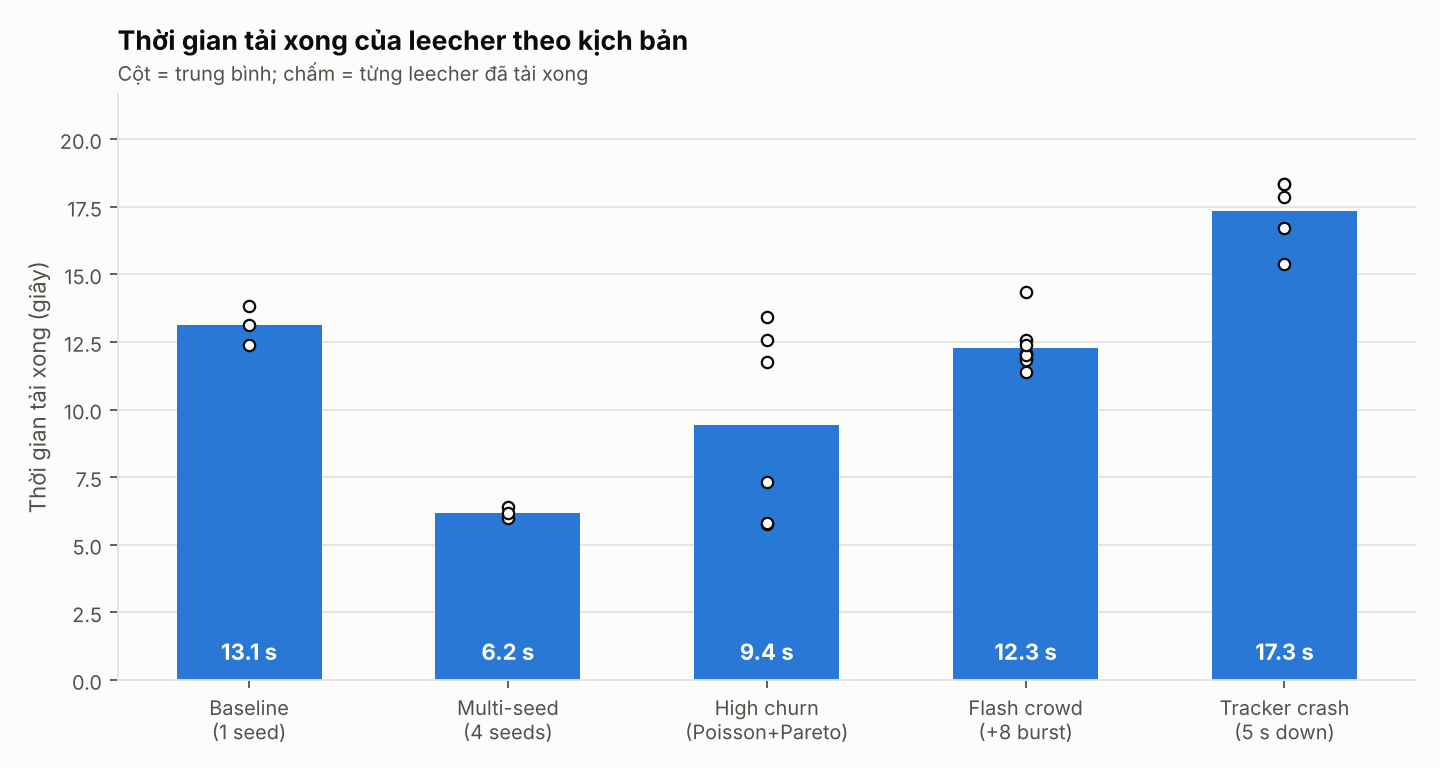
\includegraphics[width=0.92\textwidth]{images/exp1_download_time.png}
\caption{Thời gian tải của các leecher theo từng kịch bản}
\label{fig:dltime}
\end{figure}

\begin{figure}[H]
\centering
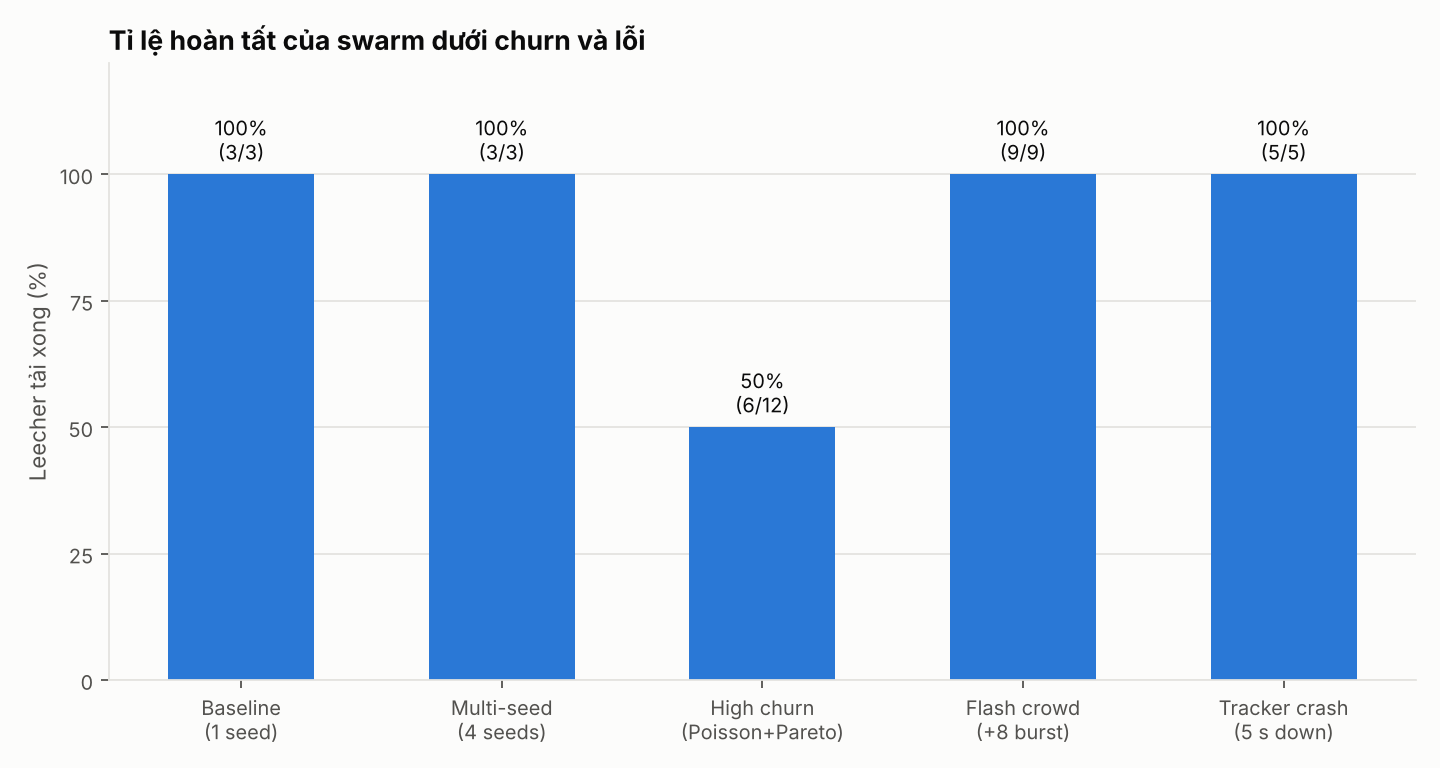
\includegraphics[width=0.85\textwidth]{images/exp2_completion_ratio.png}
\caption{Tỉ lệ leecher tải xong theo từng kịch bản}
\end{figure}

\subsection{Baseline}
Cả 3 leecher đều tải xong, trung bình 13.1 s. Điều đáng chú ý là \textbf{44\%} dữ liệu được phục vụ bởi chính các leecher chứ không phải seed. Dù seed chỉ có 256 KiB/s, các leecher trao đổi chunk cho nhau ngay khi có nên thông lượng đỉnh của cả swarm lên tới 1280 KiB/s -- đây đúng là ưu điểm của P2P.

\subsection{Multi-seed}
Với 4 seed, thời gian tải giảm còn 6.2 s, \textbf{nhanh hơn 2.12 lần} so với baseline. Tốc độ không tăng đủ 4 lần vì ở baseline các leecher đã bù một phần băng thông, và mỗi chunk vẫn có một độ trễ cố định không giảm theo số seed. Tỉ lệ leecher upload giảm còn 8\% vì seed đã đủ nhanh.

\subsection{High churn}
Có 12 leecher tham gia, trong đó nhiều peer bị kill đột ngột. Hệ thống ghi nhận \textbf{20 lần} \texttt{peer\_lost} và \textbf{8 lần} \texttt{switch\_source}: peer phát hiện nguồn chết và tự chuyển sang nguồn khác, các leecher tĩnh vẫn tải xong đúng hash. Tỉ lệ hoàn tất chỉ đạt 50\% vì phân phối Pareto có nhiều peer sống rất ngắn, rời mạng trước khi kịp tải đủ -- đây là hành vi mong đợi, không phải lỗi. Do seed gốc luôn online nên mọi chunk luôn có ít nhất 1 bản sao.

\subsection{Flash crowd}
8 leecher ập vào cùng lúc nhưng vẫn hoàn tất 100\%, trung bình 12.3 s. Leecher phục vụ tới \textbf{82\%} dữ liệu: một seed không đủ băng thông cho cả đám đông, nhưng rarest-first giúp các leecher giữ những chunk khác nhau nên có thể trao đổi cho nhau. Tracker chịu tải đỉnh 13 announce/giây.

\begin{figure}[H]
\centering
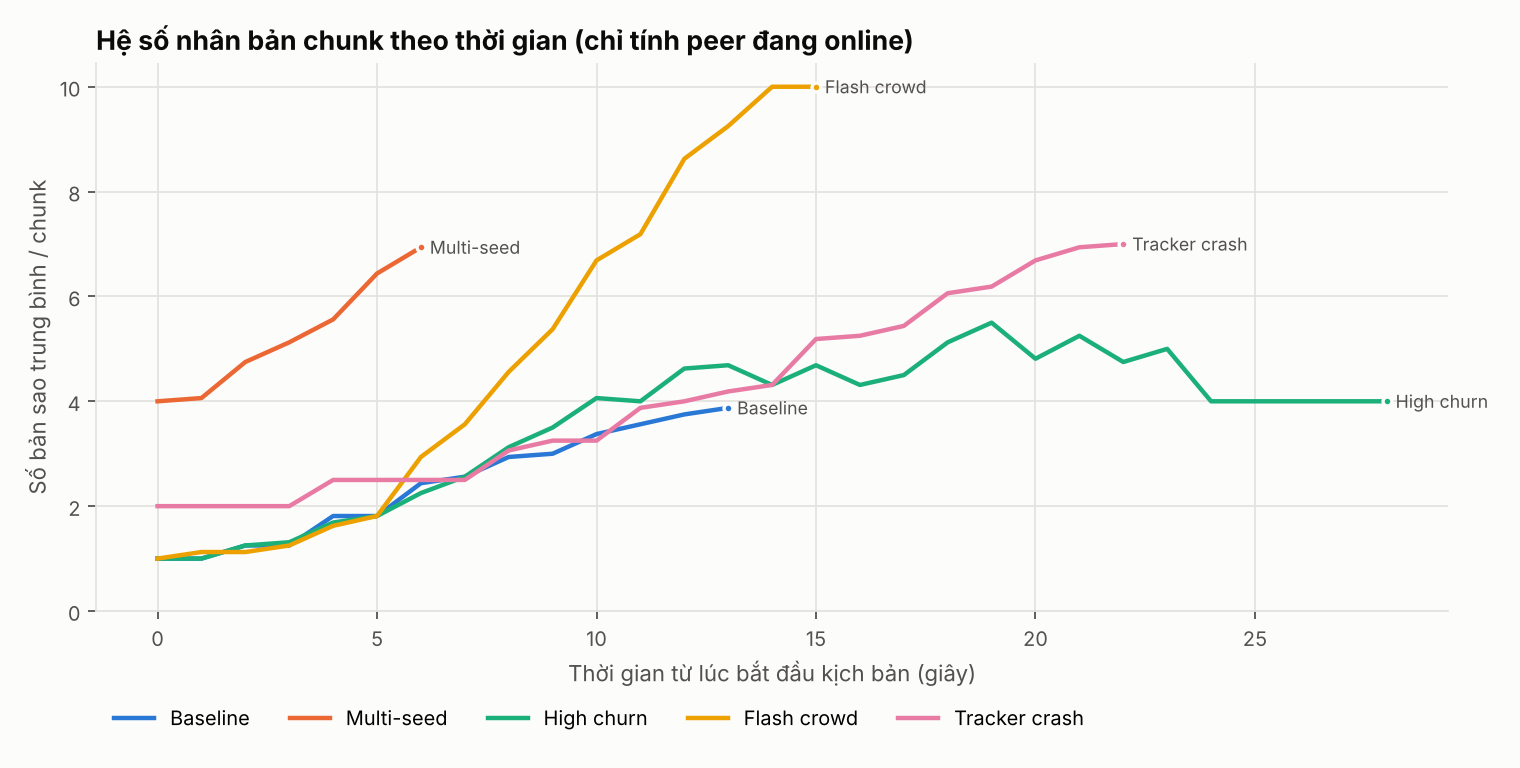
\includegraphics[width=0.92\textwidth]{images/exp3_chunk_replication.png}
\caption{Hệ số nhân bản trung bình của chunk theo thời gian}
\label{fig:replication}
\end{figure}

Hình~\ref{fig:replication} cho thấy số bản sao của chunk tăng nhanh sau đợt ập vào và sụt mạnh khi các peer rời đồng loạt. Seed gốc là điều kiện để không chunk nào biến mất hoàn toàn.

\subsection{Tracker crash}
Tracker ngừng hoạt động khoảng 5.1 s, trong thời gian đó có 27 lần announce thất bại. Tuy vậy, tỉ lệ hoàn tất vẫn là \textbf{100\%}: các peer đã biết nhau vẫn trao đổi chunk trực tiếp. Hai leecher đến lúc tracker đang sập không tìm được nguồn cho tới khi tracker sống lại (nhờ announce thử lại với backoff). Sau khi tracker khởi động lại, swarm được đăng ký lại đầy đủ sau khoảng 1.5 s mà tracker không cần lưu bất kỳ trạng thái nào.

\begin{figure}[H]
\centering
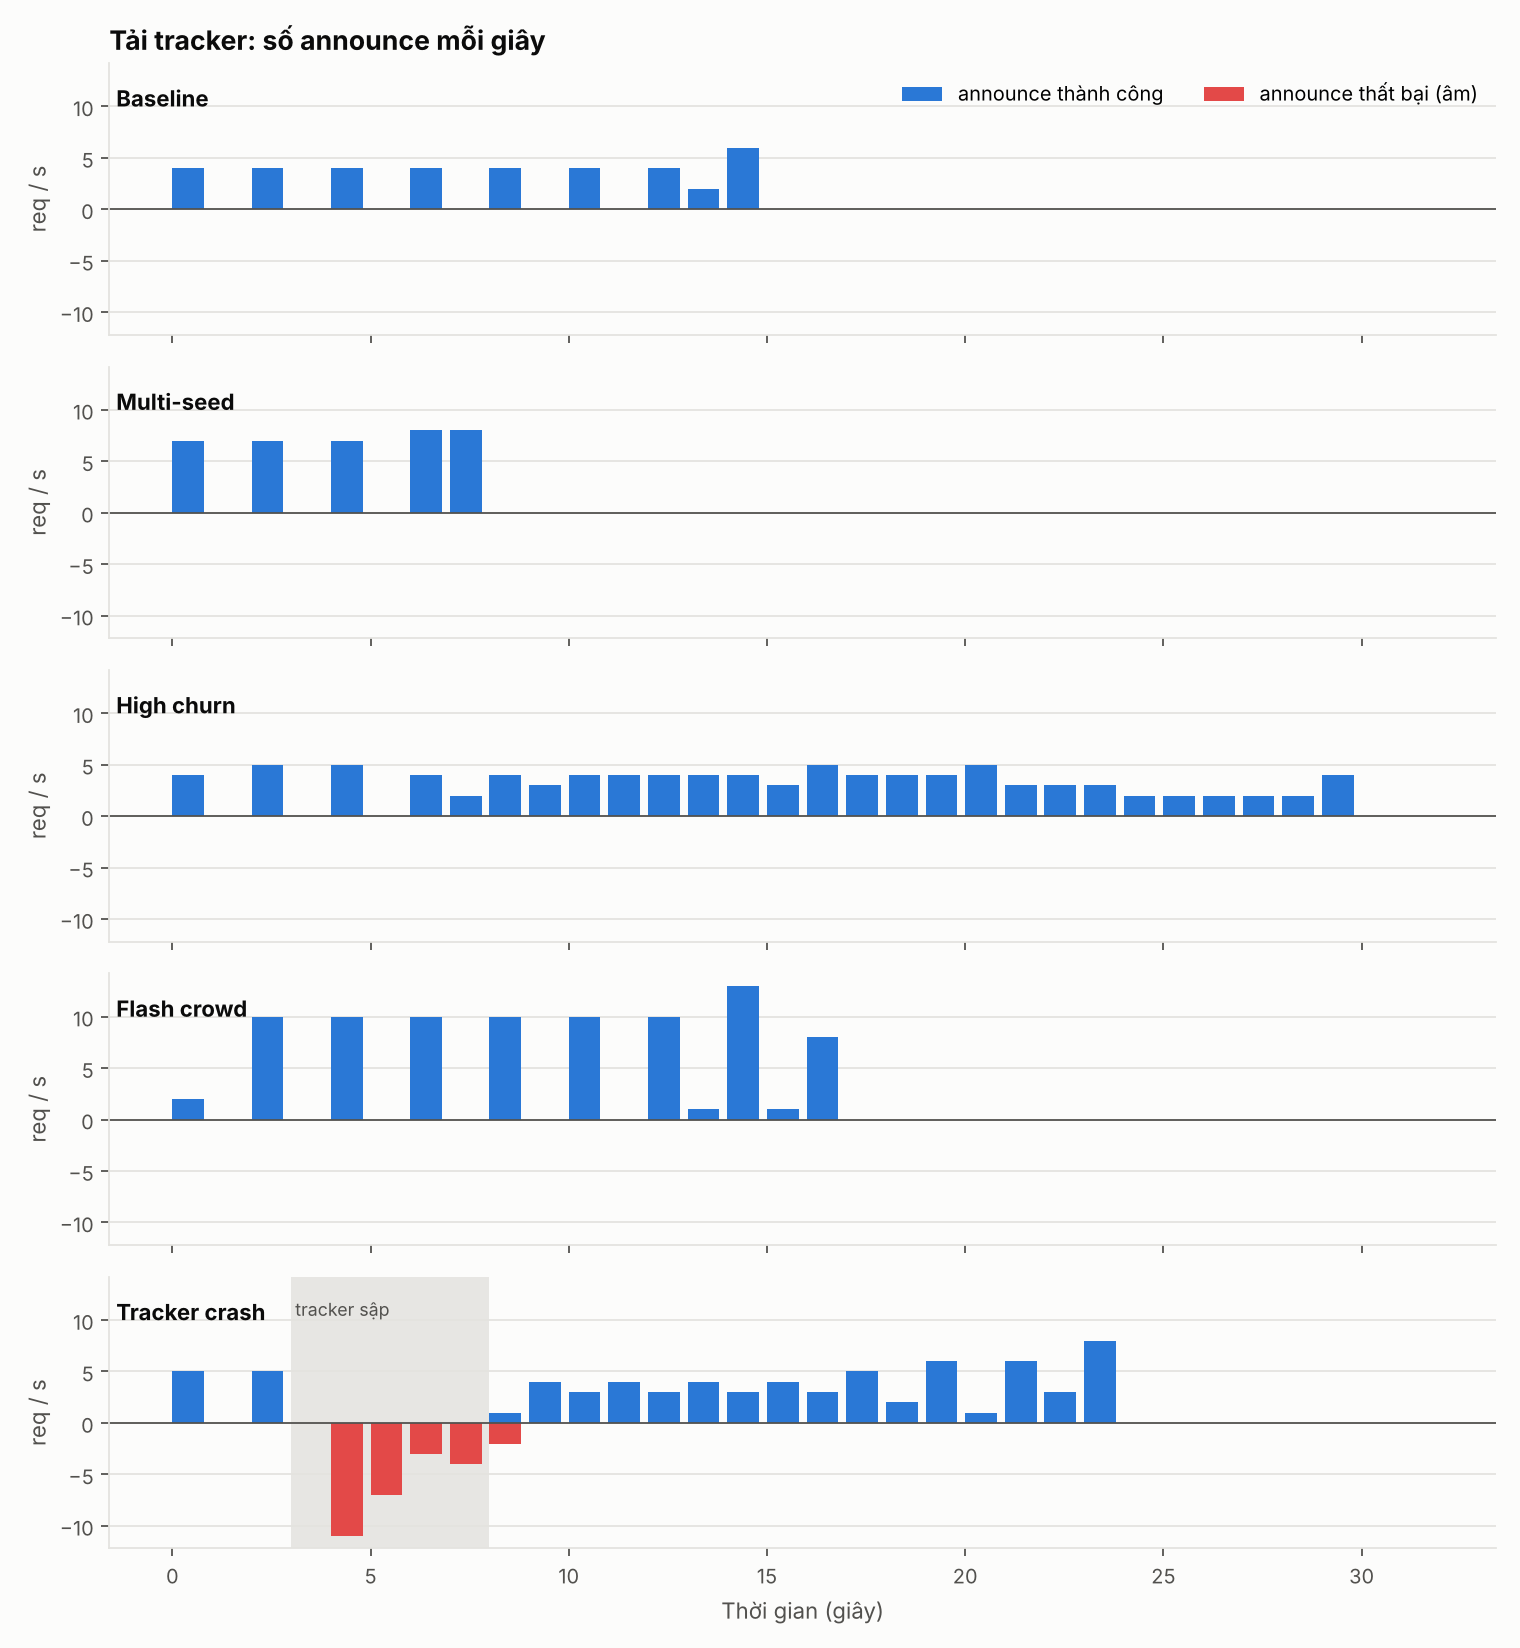
\includegraphics[width=0.92\textwidth]{images/exp5_tracker_load.png}
\caption{Số announce tới tracker mỗi giây (đánh dấu khoảng tracker sập)}
\end{figure}

\begin{figure}[H]
\centering
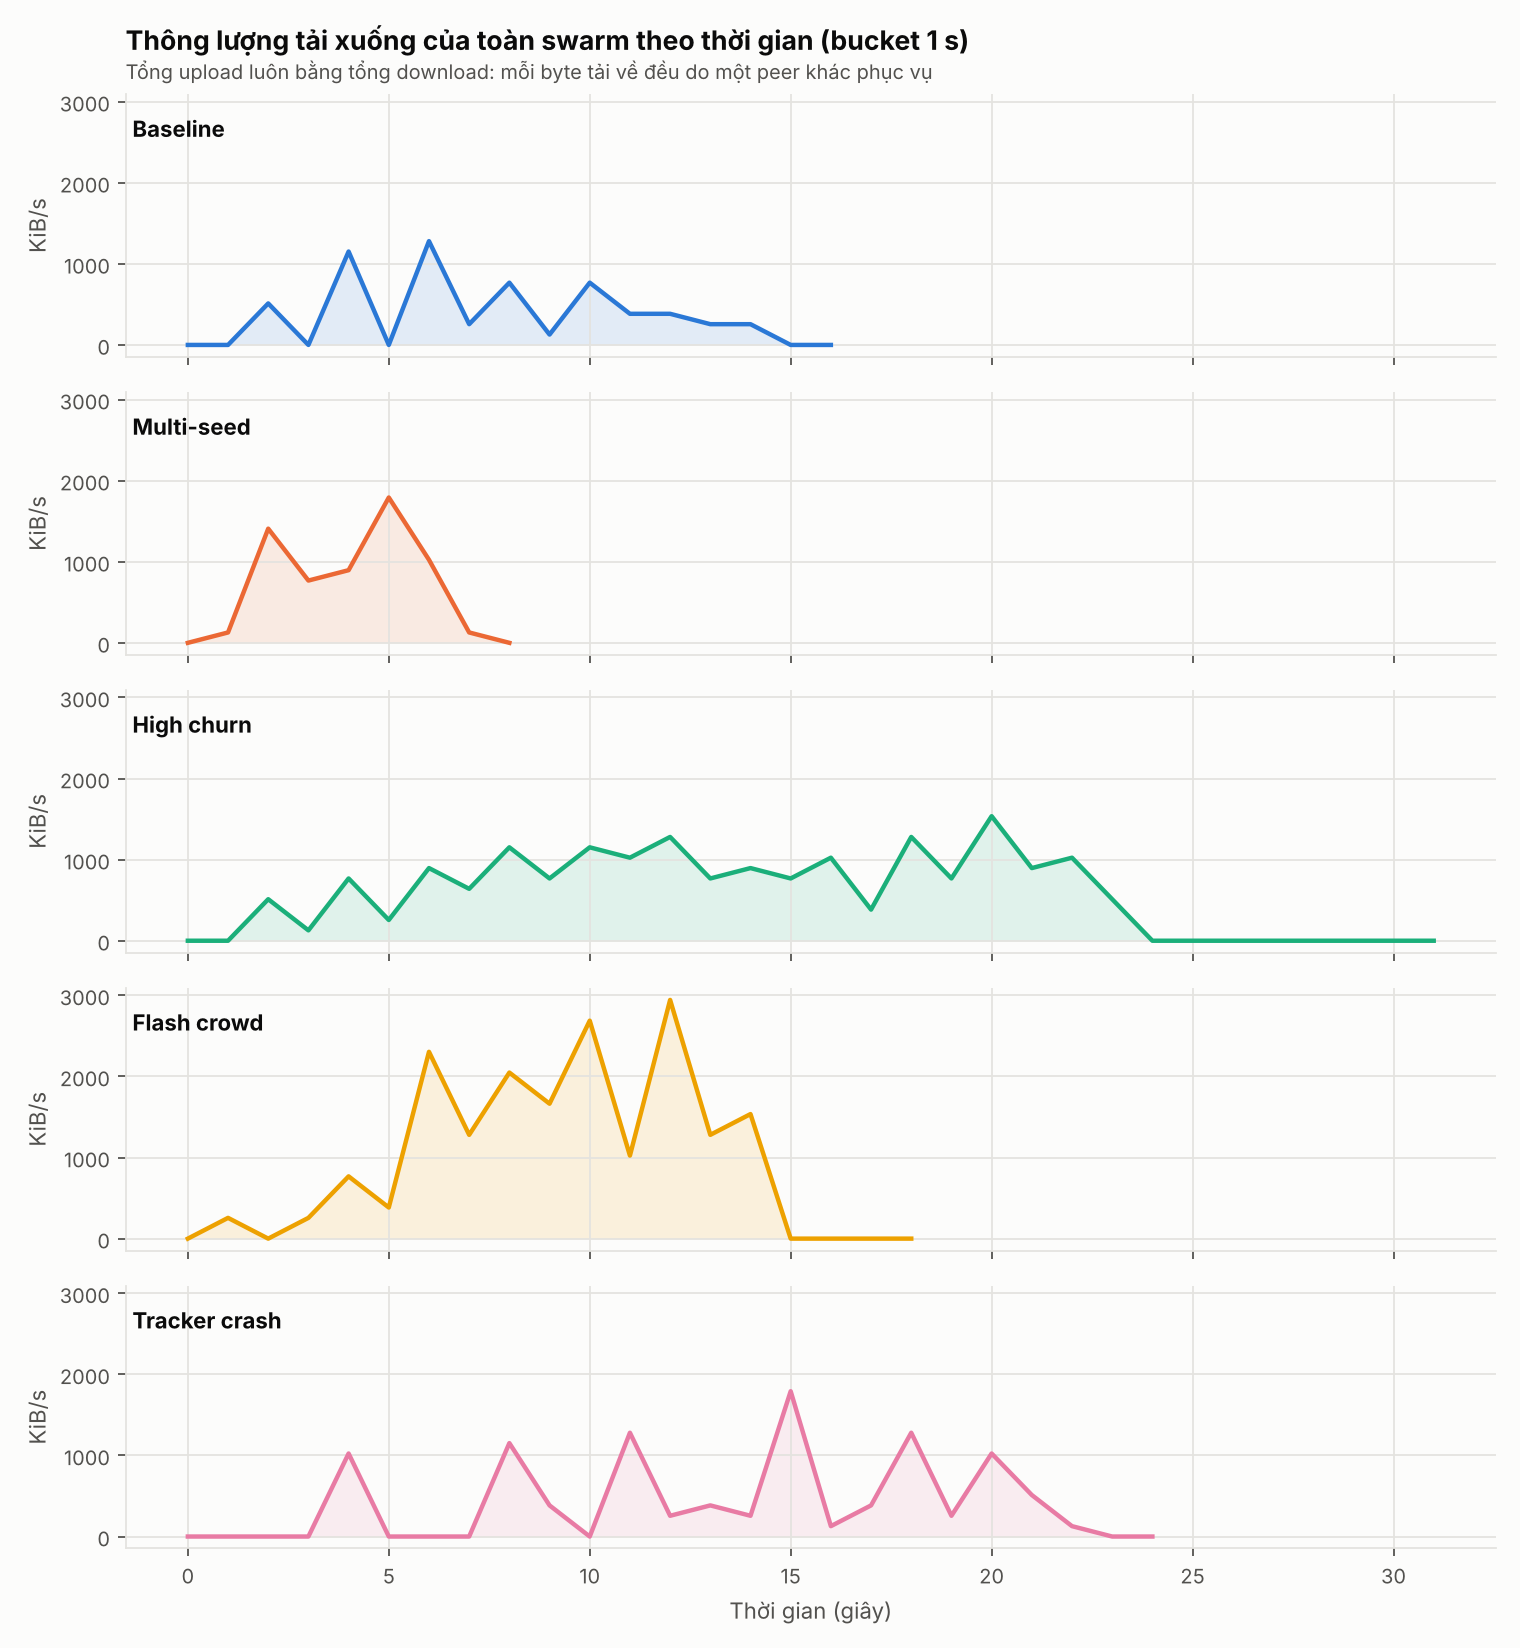
\includegraphics[width=0.92\textwidth]{images/exp4_throughput.png}
\caption{Thông lượng tải xuống / tải lên của swarm theo thời gian}
\end{figure}

\begin{figure}[H]
\centering
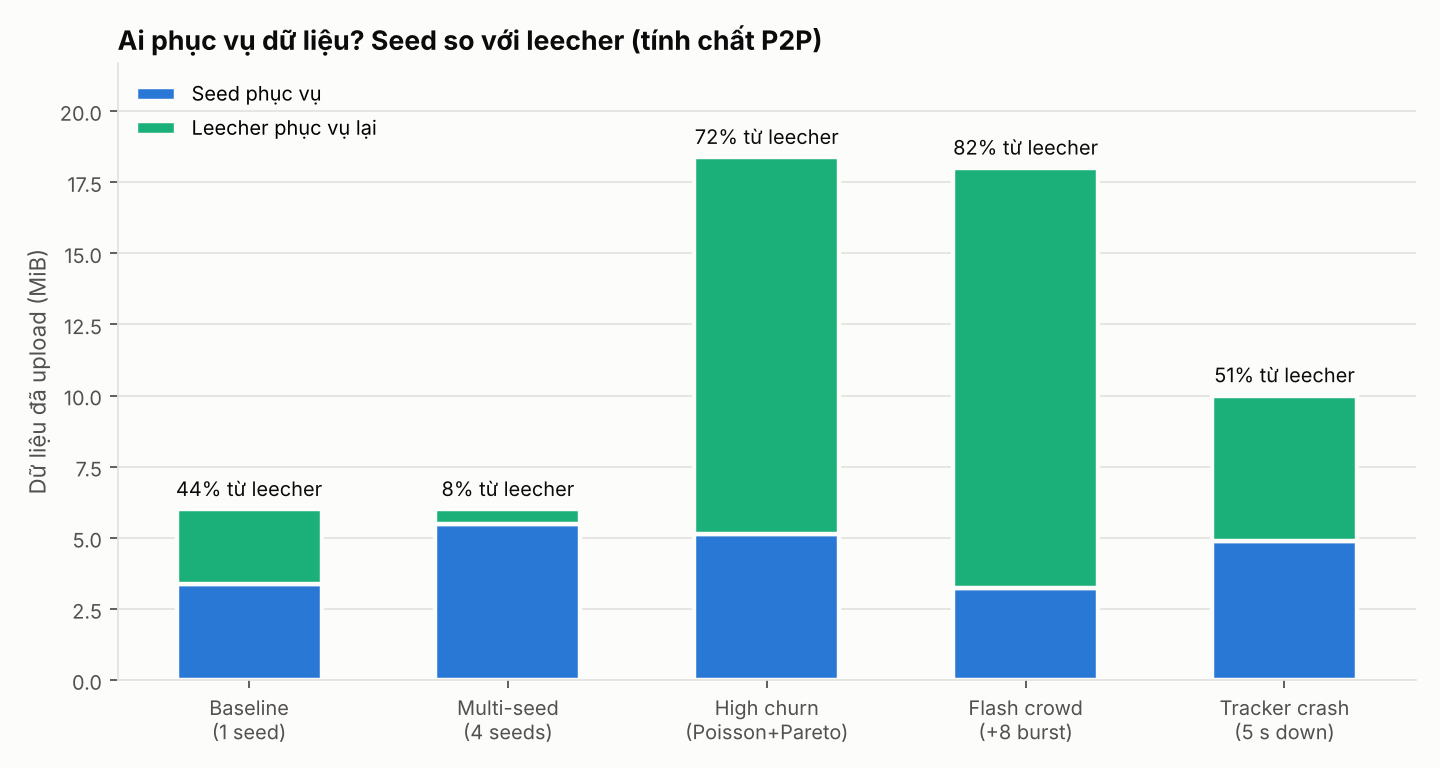
\includegraphics[width=0.85\textwidth]{images/exp6_upload_share.png}
\caption{Tỉ lệ dữ liệu do seed và do leecher phục vụ}
\end{figure}

\section{Đo tải tracker}

Nhóm dùng script \texttt{scripts/benchmark\_tracker.py} gửi 500 request \texttt{announce} với 20 luồng song song tới tracker thật trên loopback:

\begin{table}[H]
\centering
\caption{Kết quả đo tải tracker}
\begin{tabular}{@{}lr@{}}
\toprule
\textbf{Chỉ số} & \textbf{Giá trị}\\\midrule
Tổng số request & 500\\
Số luồng đồng thời & 20\\
Thông lượng & 589.0 request/s\\
Tỉ lệ thành công & 100\% (0 lỗi)\\
Độ trễ trung bình & 25.54 ms\\
Độ trễ p50 / p95 & 4.02 ms / 10.84 ms\\
Độ trễ p99 / max & 667.69 ms / 672.94 ms\\
\bottomrule
\end{tabular}
\end{table}

Phần lớn request được xử lý dưới 11 ms. Một số ít request có độ trễ cao (p99) do hàng đợi kết nối của socket bị đầy trong đợt đầu, khi 20 luồng cùng mở kết nối mới. Với quy mô vài chục peer announce mỗi 2 giây như trong thí nghiệm thì tracker dư sức đáp ứng.

\section{Demo}
Lệnh \texttt{py demo/run\_demo.py} chạy khoảng 30 giây và kiểm tra đủ 7 tình huống bắt buộc của đề: (1) tạo metadata và chia sẻ; (2) tải song song từ ít nhất 2 peer; (3) leecher upload trước khi tải xong; (4) dừng một nguồn giữa chừng; (5) tự chuyển nguồn; (6) phát hiện và từ chối chunk sai hash; (7) ghép file và xác minh hash. Kết quả: \texttt{RESULT: 7/7}.

% ================================================================= CHƯƠNG 6
\chapter{Kết luận và hướng phát triển}

\section{Kết quả đạt được}
\begin{itemize}
  \item Xây dựng hoàn chỉnh hệ thống chia sẻ file P2P kiểu BitTorrent gồm tracker, peer và bộ mô phỏng; các thành phần chạy như tiến trình riêng và giao tiếp qua mạng thật.
  \item \textbf{Tính đúng:} trong mọi kịch bản, leecher báo \texttt{completed} đều có file trùng SHA-256 với file gốc; chunk sai hash luôn bị từ chối.
  \item \textbf{Hiệu năng:} tăng khi thêm nguồn (multi-seed nhanh hơn 2.12 lần) và nhờ leecher phục vụ lại (tới 82\% dữ liệu trong flash crowd).
  \item \textbf{Chịu lỗi:} mất nguồn thì tự đổi nguồn; tracker sập không làm gián đoạn việc trao đổi chunk; swarm tự dựng lại sau khi tracker khởi động lại.
  \item Có bộ kiểm thử tự động, pipeline thí nghiệm sinh CSV/biểu đồ và demo một lệnh.
  \item Về làm việc nhóm: cách ``chốt hợp đồng trước, mỗi người tự viết mock'' giúp ba người làm song song gần như không phải chờ nhau, và việc tích hợp cuối cùng chỉ là đổi tham số dòng lệnh.
\end{itemize}

\section{Hạn chế}
\begin{itemize}
  \item Mọi thứ chạy trên một máy (loopback) nên độ trễ và băng thông là giả lập, chưa phản ánh hết mạng thật (mất gói, NAT, tường lửa).
  \item Tracker vẫn là thành phần tập trung: peer mới không thể tham gia khi tracker sập.
  \item Chỉ giới hạn băng thông chiều upload; cơ chế choke còn đơn giản (chưa có tit-for-tat và optimistic unchoke như BitTorrent gốc).
  \item Metainfo dùng JSON thay vì bencode nên không tương thích với client BitTorrent thật.
  \item Kết quả thời gian có dao động nhỏ giữa các lần chạy do lập lịch luồng của hệ điều hành (lịch churn thì tất định).
\end{itemize}

\section{Hướng phát triển}
\begin{itemize}
  \item Thêm DHT (Kademlia) để tìm peer không cần tracker, hoặc hỗ trợ nhiều tracker dự phòng.
  \item Cài đặt choking theo tit-for-tat và optimistic unchoke để khuyến khích chia sẻ công bằng.
  \item Chạy thử trên nhiều máy thật hoặc dùng \texttt{tc netem} / Docker để giả lập mạng chính xác hơn.
  \item Hỗ trợ torrent nhiều file, định dạng bencode và magnet link để tương thích với client thật.
  \item Mã hóa kết nối giữa các peer.
\end{itemize}

% ================================================================= TÀI LIỆU
\begin{thebibliography}{9}
\addcontentsline{toc}{chapter}{Tài liệu tham khảo}
\bibitem{tanenbaum} A. S. Tanenbaum, M. van Steen, \textit{Distributed Systems}, 4th ed., distributed-systems.net, 2023.
\bibitem{bep3} B. Cohen, ``The BitTorrent Protocol Specification (BEP 3)'', bittorrent.org, 2008.
\bibitem{cohen03} B. Cohen, ``Incentives Build Robustness in BitTorrent'', \textit{Workshop on Economics of Peer-to-Peer Systems}, 2003.
\bibitem{legout} A. Legout, G. Urvoy-Keller, P. Michiardi, ``Rarest First and Choke Algorithms Are Enough'', \textit{ACM IMC}, 2006.
\bibitem{stutzbach} D. Stutzbach, R. Rejaie, ``Understanding Churn in Peer-to-Peer Networks'', \textit{ACM IMC}, 2006.
\bibitem{kademlia} P. Maymounkov, D. Mazières, ``Kademlia: A Peer-to-Peer Information System Based on the XOR Metric'', \textit{IPTPS}, 2002.
\bibitem{python} Python Software Foundation, \textit{Python 3 Documentation} -- \texttt{socket}, \texttt{asyncio}, \texttt{threading}, \texttt{http.server}, docs.python.org.
\end{thebibliography}

\end{document}
